\chapter{Marco te\'orico}\label{capit:cap2}
\vspace{-2.0325ex}%
\noindent
\rule{\textwidth}{0.5pt}
\vspace{-5.5ex}% 
\newcommand{\pushline}{\Indp}% Indent puede ir o no :p


\section{Detección rápida de objetos usando características simples utilizando el clasificador de cascada impulsada}\label{Detec}

El m\'etodo  desarrollado por (ref Viola Jones) fue creado originalmente para atacar el problema de detección de rostros, pero este puede ser usando para detectar cualquier objeto, debido a la forma en que este fue creado, pues detecta un objeto clasificando imágenes basándose en el valor de características simples.

La técnica clasifica si el objeto se encuentra en la escena, usando AdaBoost en forma de cascada, y discrimina el objeto tomando en cuenta el valor de las características, se usan las características Haar, el valor de estas es calculado mediante una imagen integral.

En seguida se explica a detalle cada etapa del método. 

\subsection{Características Haar}

\subsection{Imagen integral} 

\subsection{Clasificador AdaBoost}  

\subsection{Clasificador AdaBoost en Cascada} 




\begin{figure}%[htbp]
\centering
\subfigure[Mi metus, sed bibendum ligula efficitur eu.]{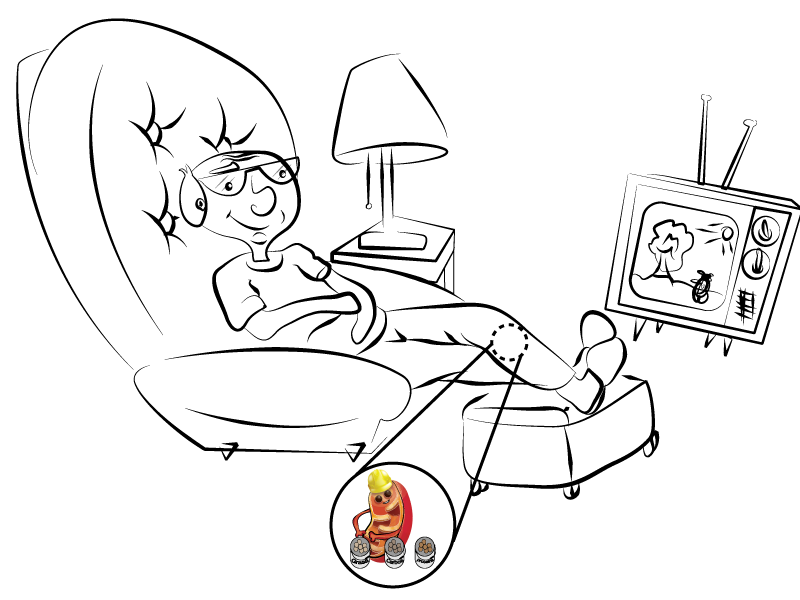
\includegraphics[width=80mm]{./Figures/instauracionFatigaReposo_1_3}} 
\subfigure[Mi metus, sed bibendum ligula efficitur eu.]{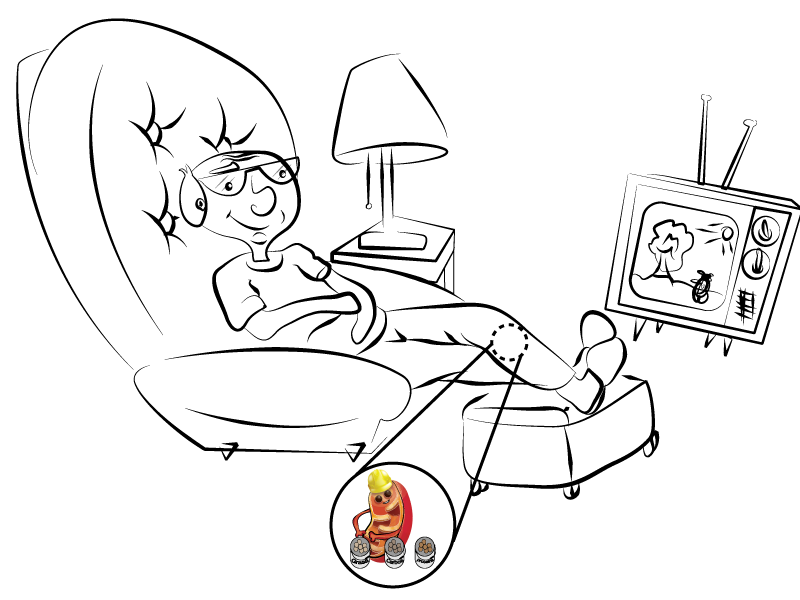
\includegraphics[width=80mm]{./Figures/instauracionFatigaReposo_1_3}}
\subfigure[Mi metus, sed bibendum ligula efficitur eu.]{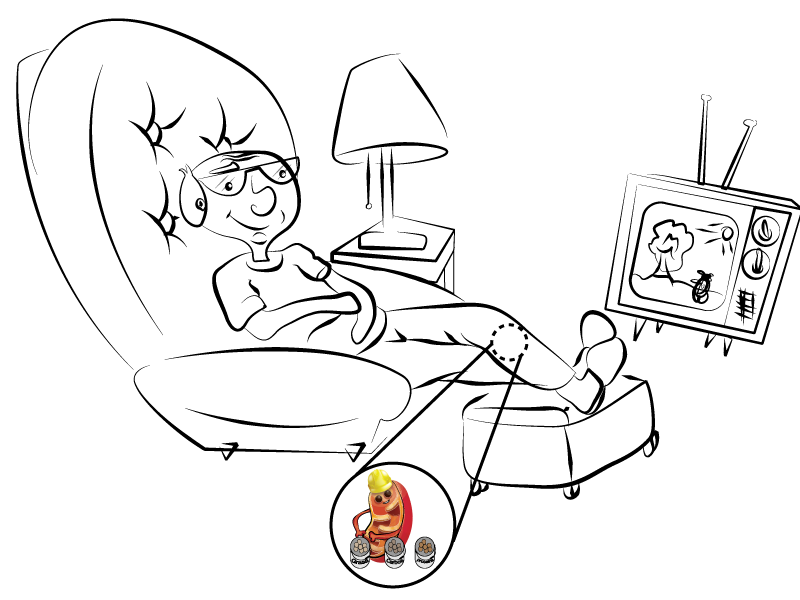
\includegraphics[width=160mm]{./Figures/instauracionFatigaReposo_1_3}}
\caption{Lorem ipsum dolor sit amet, consectetur adipiscing elit. Aliquam sit amet lobortis turpis. Praesent auctor mi metus.  } \label{fig:instauracionFatigaReposo}
\end{figure}





\newpage
%%=====================================================
